%
%
%		Finding: Template
%		Author: the DR
%
%
\renewcommand{\FindingAuthor}{Michal Olencin}
% DO NOT USE \par, \newline or any other line breaking command in FindingName => report will not build
\renewcommand{\FindingName}{Heap Inspection of Sensitive Memory}
\renewcommand{\Location}{dummyapplication.apk, dummyapplication.ipa}
\renewcommand{\Component}{AppCacheTemplate}
\renewcommand{\FoundWith}{Manual testing}
\renewcommand{\TestMethod}{Manual}
\renewcommand{\CVSS}{3.3}
\renewcommand{\CVSSvector}{CVSS:3.1/AV:L/AC:L/PR:L/UI:N/S:U/C:L/I:N/A:N}
\renewcommand{\CWE}{244}
% Poor-man's combo boxes:
% High, Medium, Low, Info, TBR (To Be Rated)
\renewcommand{\Criticality}{Low}
% Easy, Average, Hard, TBR (To Be Rated)
\renewcommand{\Exploitability}{Average}
% Access control, Application Design, Information Disclosure, Outdated Software, Security Configuration
\renewcommand{\Category}{Undefined}
% Easy, Average, Difficult, TBR (To Be Rated)
\renewcommand{\Detectability}{Easy}


\ReportFindingHeader{\FindingName}


%-------------------------------------------
%	Details                                |
%-------------------------------------------

\subsection*{Details}

The unprotected in-memory storage of plaintext sensitive data exposes its contents to potential disclosure.
An absence of secure deletion mechanisms further extend the attack surface past the necessary longevity of the contents.


%-<Details>
%-------------------------------------------
%	Impact                                 |
%-------------------------------------------



\subsection*{Impact}

Sensitive data residing in memory could be exposed to an attacker during a "heap inspection" attack.
For instance, plaintext account credentials could be exposed during the exploitation of a memory disclosure vulnerability or the execution of a memory dump.

%-<Impact>
%-------------------------------------------
%	Repeatability                          |
%-------------------------------------------
\pagebreak


\subsection*{Repeatability}

By using static analysis, one can observe the variable \texttt{pJwt} is stored as \texttt{string} type in the \texttt{AppCacheTemplate} (see \cref{figure:code}).

\begin{figure}[H]
\centering
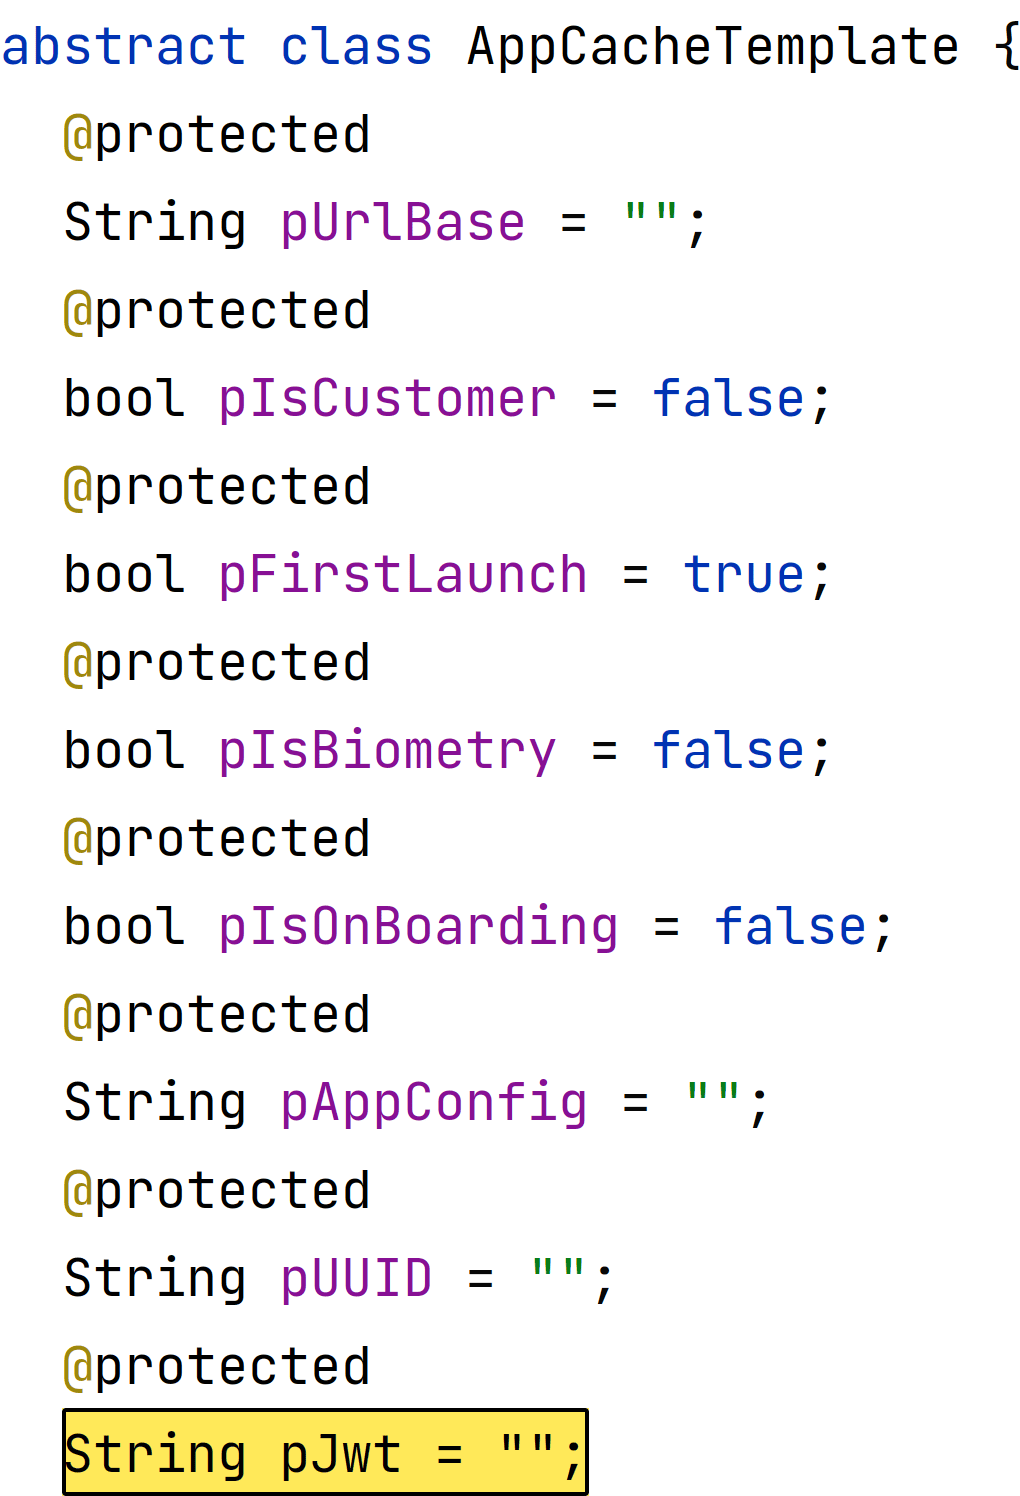
\includegraphics[width=0.4\textwidth,frame]{\CurrentFilePath/code.png}
\caption{Snippet of the \texttt{AppCacheTemplate} class}
\label{figure:code}
\end{figure}

By following the following steps, contents of the \texttt{pJwt} variable can be read from memory:

\begin{enumerate}
    \item Click \textbf{View} > \textbf{Tool Windows} > \textbf{Profiler} in the Android Studio.
    \item Select the device and app process.
    \item In memory profiler capture the memory dump (see \cref{figure:dump}).
    \item Extract a JWT from memory (see \cref{figure:extract}).
\end{enumerate}

 \begin{figure}[H]
 \centering
 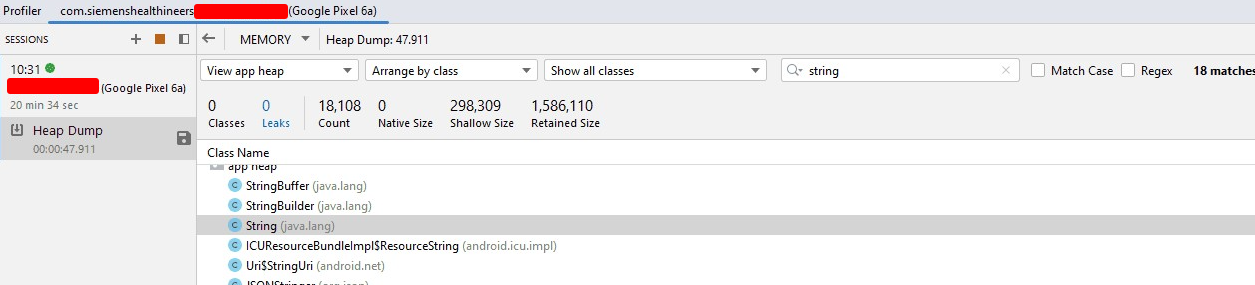
\includegraphics[width=1\textwidth,frame]{\CurrentFilePath/dump.png}
 \caption{Capturing the memory dump}
 \label{figure:dump}
 \end{figure}

 \begin{figure}[H]
 \centering
 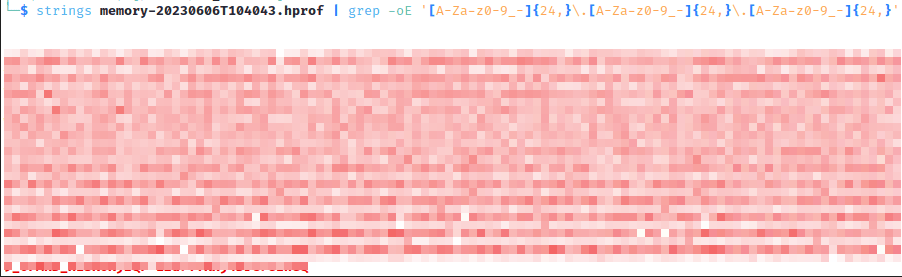
\includegraphics[width=1\textwidth,frame]{\CurrentFilePath/extract.png}
 \caption{Extracting a JWT from memory}
 \label{figure:extract}
 \end{figure}

%-<Repeatability>
%-------------------------------------------
%	Countermeasures                        |
%-------------------------------------------



\subsection*{Countermeasures}

As countermeasure, don't save JWT to variable in the \texttt{AppCacheTemplate} class.
Instead, directly access JWT value form \texttt{FlutterSecureStorage} instance.

Review source code for storing sensitive data in memory.
Substitute ordinary \texttt{String} objects with \texttt{byte[]}, which can be cleared from memory when no longer needed.
However, it is important to ensure that the \texttt{byte[]} is securely encrypted and cleared from memory when no longer needed to prevent sensitive information from being disclosed.

%-<Countermeasures>
%-------------------------------------------
%	References - pulls bib entries         |
%-------------------------------------------



\subsection*{References}

This finding references the following information sources:

\begin{itemize}
	\item \href{https://www.first.org/cvss/calculator/3.1#CVSS:3.1/AV:L/AC:L/PR:L/UI:N/S:U/C:L/I:N/A:N}{CVSS 3.3}
    \item \href{https://developer.android.com/studio/profile/memory-profiler}{Memory Profiler}
	\item \bibentry{CWE-244}
\end{itemize}

%-<References>



